\documentclass[a4paper,12pt]{article}
\usepackage[UTF8]{ctex}
\usepackage{tocloft}
\usepackage{graphicx}
\usepackage{caption}
\usepackage{hyperref}

% 定义图片位置
\graphicspath{{./Figure/}}

% 重定义图注
\captionsetup[figure]{name=Figure, labelsep=colon}

% 重定义目录命令,以居中显示目录标题
\renewcommand{\contentsname}{\hfill\bfseries\Large 目录\hfill}   
\renewcommand{\cftaftertoctitle}{\hfill}

% hyperref 设置
\hypersetup{
    colorlinks=false,    % 使用边框而不是颜色链接
    pdfborderstyle={/S/U/W 0} % 无边框
}

% 定义一个用于图表引用的命令,仅为引用添加红色边框
\newcommand{\figref}[1]{%
    \begingroup
    \hypersetup{pdfborderstyle={/S/S/W 1}, linkbordercolor={1 0 0}} % 方框样式,红色
    \ref{#1}%
    \endgroup
}

\begin{document}
% 更改封面的字体样式
\title{\huge My Test Document}
\author{{\large knight-zzm}}
\date{\today}
\maketitle
\thispagestyle{empty} % 封面页无页码
\newpage

\tableofcontents
\thispagestyle{empty} % 无页码
\newpage
\pagenumbering{arabic}
\section{练习latex 论文写作}
This is the introduction.

\subsection{图表的创建和引用}
    The above data is combined to form a correlation heat map between features, as shown in Fig.\figref{fig:time-freq}
    \begin{figure}[h]
        \centering
        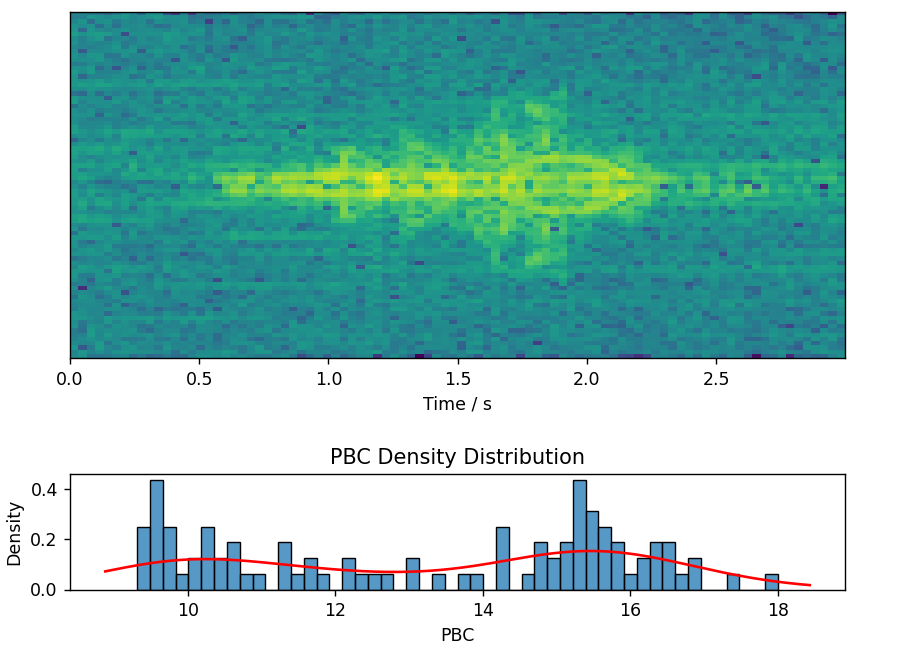
\includegraphics[width=1\textwidth]{时频图和PBC分布图.png}
        \caption{时频图和PBC分布图}
        \label{fig:time-freq}
    \end{figure}

\subsection{公式编辑和引用}

\subsection{表格编辑和引用}
    % ... [其他表格代码] ...

\end{document}
